\documentclass[
    12pt,
    oneside,
    a4paper,
    english,
    brazil
]{abntex2}

\usepackage{lmodern}
\usepackage[T1]{fontenc}
\usepackage[utf8]{inputenc}
\usepackage{indentfirst}
\usepackage{color}
\usepackage{graphicx}
\usepackage{microtype}
\usepackage{amsfonts}
\usepackage{csquotes}

\usepackage{tikz}
\usetikzlibrary{positioning}

\usepackage{caption}

\usepackage[brazilian,hyperpageref]{backref}
\usepackage[alf]{abntex2cite}

\usepackage{macros}

\titulo{Previsão de séries temporais por meio de aprendizado de máquina}
\autor{Guilherme Chichanoski}
\local{Maringá}
\data{2018}
\orientador{Valéria Delisandra Feltrim}
\instituicao{Universidade Estadual de Maringá\\
Centro de Tecnologia --- Departamento de Informática\\
Bacharelado em Ciência da Computação}
\tipotrabalho{Trabalho de Conclusão de Curso}

\preambulo{Trabalho de Conclusão de Curso de Graduação apresentado ao
Departamento de Informática da Universidade Estadual de Maringá, como requisito
parcial para obtenção do grau de Bacharel em Ciência da Computação.}

\makeatletter
\hypersetup{
    pdftitle={\@title},
    pdfauthor={\@author},
    pdfsubject={\imprimirpreambulo},
    pdfcreator={LaTeX with abnTeX2},
    pdfkeywords={séries temporais}{arima}{aprendizado de máquina}{redes neurais},
    colorlinks=true,        % false: boxed links; true: colored links
    linkcolor=red,         % color of internal links
    citecolor=green,         % color of links to bibliography
    filecolor=magenta,      % color of file links
    urlcolor=blue,
    bookmarksdepth=4
}
\makeatother

\setlength{\parindent}{1.3cm}
\setlength{\parskip}{0.2cm}

\begin{document}

\frenchspacing

\imprimircapa{}

\imprimirfolhaderosto{}

\begin{resumo}
    % TODO: Resumo

    \textbf{Palavras-chave}: séries temporais, arima, aprendizado de máquina,
    redes neurais.
\end{resumo}

\begin{resumo}[Abstract]
    \begin{otherlanguage*}{english}
        % TODO: Abstract

        \textbf{Keywords}: time series, arima, machine learning, neural
        networks.
    \end{otherlanguage*}
\end{resumo}

\textual{}

\pdfbookmark[0]{\contentsname}{toc}
\tableofcontents*
\cleardoublepage{}

\chapter{Introdução}

%VALERIA: Evite usar a 1a pessoa no texto ("podemos..., fizemos...", etc.). Embora essa forma seja comum na escrita científica em inglês, em português não é usual. Eu já corrigi essa questão em toda a parte revisada (até o início dos modelos probabilísticos). Por favor, corrija no restante.

Segundo \citeonline{wiley} prever é a capacidade de predizer valores ou eventos futuros e constitui uma tarefa de grande importância para diversos setores, incluindo governos e
industrias. Uma vez que tal capacidade é parte crucial na tomada de decisão, fica evidente a necessidade de se realizar boas previsões. No entanto, fazer boas previsões pode ser uma tarefa extremamente complexa. Muitos autores e organizações já realizaram
previsões que, com o decorrer do tempo, se mostraram erradas, como no caso do The New
York Times, que previu em 1966 que existiriam somente 220.000 computadores nos Estados Unidos no ano 2000.

Ainda conforme \citeonline{wiley}, as previsões são classificadas como sendo de
curto, médio e longo prazo, sendo o prazo definido na frequência das
observações. Quando denominadas de curto prazo, são previstas poucas observações a frente do tempo atual. Já previsões de médio prazo podem se estender por algumas observações no futuro. Por fim, previsões que envolvem um período maior no futuro são chamadas de longo prazo. Ainda
conforme o autor, predições de médio e longo prazo são mais difíceis de se realizar e suscetíveis a fatores externos.

% FIXME Acredito que deveria estar nos trabalhos relacionados
%Em \citeonline{giebel2011state} o autor realiza a predição da geração de
%energia eólica, a produção é dada em função da capacidade na região instalada,
%o vento, no entanto, é um elemento volátil e sendo assim existirá momentos
%quais o uso de outras fontes será necessária, contudo, é preciso ter certo
%conhecimento prévio, pois, o ligamento de uma usina como aquelas movidas a
%gasóleo podem levar até duas horas. Logo prever duas horas a frente pode ser
%crucial para garantir o abastecimento de energia a uma região, podendo
%impactar no cotidiano e economia de uma população.

Para a realização da previsão é necessária a compreensão do evento que se quer prever. Quando existe uma relação temporal entre as observações do evento em questão, i.e., o evento ocorre em uma determinada sequência no tempo, é necessário organizar as informações de forma a evidenciar a dependência das observações com seus estados anteriores. Nesse caso, as observações passadas compõem uma série temporal, a partir da qual é possível realizar medições e produzir modelos capazes de expressar
matematicamente o comportamento da série em função de suas observações anteriores, permitindo assim a predição de estados futuros.


% FIXME: Tá esquisito 
% VALERIA: não está claro o que vc quer mostrar com essa figura! O que vc quer que o leitor observe? Além disso, vc precisa dizer o que os eixos x e y significam.
Conforme mencionado, as séries temporais são compostas de observações sequenciais ao longo do tempo \cite{wiley}. Como exemplo, a \autoref{serie0} mostra uma série gerada utilizando-se um processo de caminhada aleatória.
Sendo essas observações separadas unicamente pelo tempo, pode-se obter os dados em diferentes intervalos, como observações diárias, semanais ou anuais.
% VALERIA: Arrumei a escrita, mas veja se é isso mesmo que vc queria dizer
Conforme \citeonline{ehlers}, devido à caraterística estocástica do processo, uma observação se define em função de suas antecessoras.

\begin{figure}[ht]
    \centering
    \caption{Série gerada para exemplo}\label{serie0}
    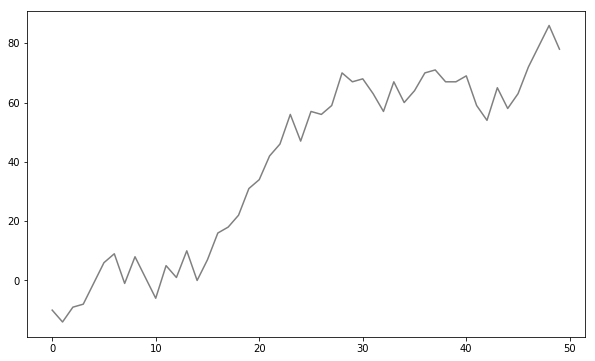
\includegraphics[width=.6\linewidth]{images/serie_exemplo.png}
    \source{Elaborado pelo autor}
\end{figure}

Considerando então que a série apresentará comportamento estocástico, é possível propor modelos que serão capazes de aproximar o comportamento da série. Os modelos comumente utilizados para essa tarefa são aqueles probabilísticos, mais especificamente o ARIMA\@, proposto por \citeonline{box}. Também é possível utilizar modelos criados a partir da aplicação de técnicas de aprendizado de máquina, que vem se apresentando como uma alternativa poderosa em
muitas aplicações.

Com o constante interesse na aplicação e a identificação das capacidades de
técnicas de aprendizado, fica evidente a importância de observar como esses modelos se comparam com os estatísticos. Dessa forma, o objetivo deste trabalho foi comparar o desempenho de modelos estatísticos e baseados em aprendizado de máquina na previsão de uma série de característica econômica. Especificamente, foram avaliados o modelo estatístico ARIMA e um modelo de aprendizado de máquina baseado em redes neurais artificiais de múltiplas camadas. Os resultados indicaram....
%VALERIA: precisa dizer qual(is) modelo(s) estatístico(s) e de aprendizado de máquina vc avaliou. Tb precisa dizer de forma sumarizada qual foi o resultado.

%Como forma de comparar desempenhos e buscar compreender as técnicas que poderiam ser utilizadas para a previsão, este trabalho realizou a previsão de uma série de característica econômica utilizando ambas metodologias.

% TODO: Introduzir modelos ARIMA com exemplos de artigos

% FIXME Mais adequado na parte de trabalhos relacionados
%vez mais notórias pelos bons resultados que oferecem. \citeonline{artigoEx3}
%Em contrapartida, técnicas de aprendizado de máquinas estão se tornando cada
%aplicou métodos de aprendizado de máquina possibilitando a previsão com bons
%resultados.  Pelo fato dos modelos estatísticos fornecerem resultados
%satisfatórios para predições e estarem bem difundidos na comunidade acadêmica,
%é comum que trabalhos como \citeonline{artigoEx4} compare os resultados
%obtidos a partir de aprendizado de máquina com modelos de abordagem
%estatísticas. Para modelos de aprendizado se destaca aqueles com uso de redes
%neurais artificiais por serem capazes de obter bons resultados conforme
%analisado por \citeonline{zhang}, o autor ainda apresenta outros exemplos
%quais os autores obtiveram resultados superiores ao método estatístico.

O restante desta monografia está organizada como segue. No \autoref{chap:fundTeor} é apresentada a fundamentação teórica do trabalho, incluindo os principais métodos de previsão de séries temporais empregados. No \autoref{chap:desenv} são descritos os passos metodológicos empregados para a desenvolvimento tanto do modelo estatístico quanto de aprendizado de máquina. Os resultados obtidos com base nos modelos construídos são apresentados no
\autoref{chap:result}. 
%VALERIA: discussão de resultados deve ficar no capítulo de resultados, não na conclusão. Na conclusão se resume o que foi feito, se indica os principais resultados e se dá as conclusões finais.
Por fim, no \autoref{chap:concl} é apresentada a discussão dos resultados, bem como as conclusões obtidas.

\chapter{Fundamentação teórica}\label{chap:fundTeor}

\section{Previsão}
Segundo \citeonline{wiley}, o processo de previsão pode ser dividido em diversas atividades, dispostas a seguir:

\begin{enumerate}
    \item Definição do problema\\
        Envolve definir e entender a tarefa de previsão a ser realizada,
        considerando o prazo a ser previsto e definindo os dados necessários.
    \item Coleta dos dados\\
        Envolve a coleta dos dados necessários de acordo com as definições da atividade anterior.
    \item Análise dos dados\\
        Atividade de alta importância para a seleção do modelo mais adequado. Nessa etapa são utilizadas observações gráficas e extração de
        características para identificar padrões que corroborem na escolha dos
        parâmetros. Também são identificadas observações problemáticas e, caso necessário, aplicadas as devidas correções.
    \item Seleção e verificação do modelo\\
        A partir da análise feita na atividade anterior, será selecionado o modelo, analisando-se também o
        comportamento com os dados fornecidos. Como método de verificação são utilizadas métricas que favoreçam a comparação.
    \item Avaliação do modelo\\
        Atividade na qual se avalia como o modelo se comporta com novos dados, normalmente realizada com observações excluídas dos dados utilizados nas atividades anteriores. As observações separadas para avaliação são utilizadas apenas para essa finalidade.
    \item Publicação do modelo\\
        Com o modelo devidamente selecionado e avaliado, o mesmo é instalado em ambiente de produção, observando-se as alterações necessárias para que novos dados sejam inseridos corretamente.
    \item Monitoramento do desempenho do modelo\\
        Deve-se continuamente avaliar como o modelo aplicado se comporta em relação ao ambiente, já que o ambiente é algo volátil.
\end{enumerate}

Essas atividades normalmente são realizadas em ordem semelhante a exposta. Vale observar ainda que se os resultados da atividade de avaliação forem insatisfatórios, deve-se retornar à atividade anterior e refazer a avaliação até que
um modelo que obedeça às especificações seja encontrado.

\section{Séries temporais}

Como exposto anteriormente, séries temporais são compostas por observações sucessivas feitas ao longo do tempo. Cabe destacar ainda que essas séries se caracterizam pelo fato de suas observações serem dependentes das observações anteriores. Além disso, tais séries demonstram características como tendência e sazonalidade. A tendência caracteriza o comportamento de crescimento/decrescimento da série, o que pode levar a observações futuras com valores menores ou maiores. A sazonalidade caracteriza padrões cíclicos em função do tempo, comumente tomando períodos semanais, mensais ou anuais.

%VALERIA: o que o T (maiúsculo) significa na definição? Achei que fosse tempo, mas no parágrafo seguinte aparece a Equação 2.1 na qual o T é usado para designar a tendência. Achei confuso.
Uma série é descrita matematicamente pelo conjunto $\{X(t): t \in T\}$, podendo
$t$ ser um tempo contínuo ou discreto. O tempo $t$ é dito contínuo quando se possui observações $X(t)$ para todo $t$ em $T$, sendo $T \subseteq
\mathbb{R}^{+}$. O tempo $t$ é discreto quando entre as observações $X(t_i)$ e $X(t_i_+_1)$ existe um intervalo igual de tempo, normalmente dado na forma de uma sequência, $T = \{1,
2, \ldots, n\}$, sendo $n$ o número de observações.

Segundo \citeonline{ehlers}, uma série temporal classicamente é decomposta
seguindo a \autoref{eq:timeseries}, sendo $t$ usado para denotar o tempo, $T$
denota a tendência, $C$ a sazonalidade, e $R$ é a componente aleatória caracterizada por possuir média zero, também denotada como ruído branco.

\begin{equation}
    \label{eq:timeseries}
    X_t = T_t + C_t + R_t
\end{equation}

\subsection{Série estacionária}

%VALERIA: tirei essa definição de um site de estatística
%http://www.portalaction.com.br/series-temporais/13-processos-estacionarios
% mas precisaria usar uma definição tirada de um livro.
Um conceito importante para a análise de séries temporais é o seu caráter estacionário. Um processo é dito estacionário se todas as suas características comportamentais não se alteram ao longo do tempo. Em outras palavras, o processo se desenvolve no tempo em torno da média, de modo que a escolha de uma origem dos tempos não é importante. Segundo \citeonline{ehlers}, uma série é dita estritamente estacionária quando a distribuição de probabilidade conjunta de $X(t_1), \ldots, X(t_k)$ é igual a de $X(t_1 + \tau), \ldots, X(t_k + \tau)$.

Ainda segundo \citeonline{ehlers}, a definição estrita de série estacionária é dificilmente aplicada, então usualmente se utiliza a definição de série fracamente estacionária, que se
define com base no critério da mesma possuir função média constante.
Dessa forma, no decorrer deste trabalho, se usará a definição de série fracamente estacionária para se tomar uma série como estacionária.

Em termos matemáticos, usa-se a \autoref{eq:westacionaria} para
definir que variância de um elemento da série ($z_t$) deve ser semelhante à média. Em outras palavras, o deslocamento da origem do tempo $t$ por uma quantidade $\tau$ não exerce efeito na distribuição conjunta da série. Assim, o valor esperado para a série em determinado momento não será dada em função do tempo.

\begin{equation}
    \label{eq:westacionaria}
    E(z_t) = \mu_t = \mu
\end{equation}

% FIXME Dada em função de que??


%TODO Adicionar referência ao Livro Time Series by exmples

%TODO Adicionar referência ao teste de Dockey Fuller

%VALERIA: Deixe para mostrar o exemplo da série estacionária pós-diferenciação na seção que fala sobre a diferenciação. Neste ponto do texto ficou fora de contexto. Ou, se vc quer mostrar um exemplo, mostre uma série originalmente estacionária. Além disso, nesse caso, vc tem que explicar melhor a figura. Por exemplo, qual(is) característica(s) do gráfico da série me diz(em) que ela é estacionária? Dizer que a observação do gráfico é suficiente não é suficiente. ;)

%A \autoref{fig:co2diff} é um exemplo de série estacionária encontrada ao aplicar o processo de diferenciação na série apresentada na \autoref{fig:co2}, este processo está descrito na \autoref{sec:diff}. Segundo \citeonline{tsExample} embora exista testes como o de Dikey Fuller descrito em \citeonline{dickey} para a prova de estacionariedade, é suficiente a observação gráfica da série. 
%%VALERIA: O que exatamente no gráfico me diz que a série é estacionária?

\subsection{Sazonalidade e tendência}

Conforme definido por \citeonline{ehlers}, a sazonalidade caracteriza repetições de comportamento de uma série em um período $s$ de tempo. A presença da sazonalidade, em geral, é
facilmente observada na representação gráfica da série, conforme exemplificado no gráfico da \autoref{fig:co2}. Nesse gráfico é apresentada uma série temporal real que registra a mudança na concentração de $CO_2$ na atmosfera. Observando o gráfico, é possível notar que há sazonalidade de periodicidade anual.
%VALERIA: Não é evidente o que caracteriza a sazonalidade no gráfico. Deixe isso claro para o leitor. O que mostra a sazonalidade é a linha em formato de "serra", i.e., em cada ano tem um pico e um vale? 

Ainda no gráfico da \autoref{fig:co2}, também é possível notar que há uma tendência de crescimento na série. Segundo \citeonline{ehlers}, não há uma definição exata de tendência, mas normalmente a mesma é associada ao comportamento de mudança das observações ao longo de um vasto período. 
%VALERIA: o que significa o alpha?
Uma série com tendência pode ser descrita como a função
apresentada na \autoref{eq:tendencia}, na qual $\alpha$ e $\beta$ são os coeficientes %de quê???
e $\epsilon_t$ é o erro. O coeficiente $\beta$ define a taxa de crescimento da série e, desse modo, $\beta$ pode ser entendido na forma $\beta = x_t - x_{t-1}$.

\begin{equation}
    \label{eq:tendencia} X_t = \alpha + \beta_t + \epsilon_t
\end{equation}

Esse entendimento de série com tendência, segundo \citeonline{ehlers}, permite encontrar uma função polinomial representativa da série na forma mostrada na \autoref{eq:tendenciaSerie}.

\begin{equation}
    \label{eq:tendenciaSerie}
    X_t = \beta_0 + \beta_1t + \beta_2t^2 + \cdots + \beta_{p}t^p + \epsilon_t
\end{equation}

% Um exemplo real de uma série temporal que apresenta tendência e
% sazonalidade é mostrado no gráfico na \autoref{fig:co2}. Essa série registra a mudança na concentração de $CO_2$ na atmosfera, sendo, portanto, uma série de característica natural. Observando o gráfico, é fácil notar a tendência de crescimento da série e sua sazonalidade de periodicidade anual.

\begin{figure}
    \centering
    \caption{Leituras de $CO_2$ na atmosfera.}\label{fig:co2}
    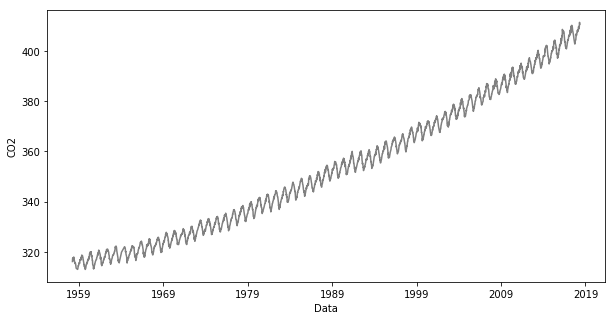
\includegraphics[width=.6\linewidth]{images/co2.png}
    \source{\citeonline{co2data}}
\end{figure}

\subsubsection{Filtros}

%VALERIA:essas flutuações seriam a sazonalidade?
Em algumas séries a tendência pode não estar evidente devido a flutuações.
Por conta disso, pode ser necessária a aplicação de filtros que têm como objetivo obter uma série suavizada que possibilite observar a tendência. 
%VALERIA: Esse filtro tem nome?
Um desses filtros é apresentado na \autoref{eq:filtro} \cite{ehlers}.

\begin{equation}
    \label{eq:filtro}
    y_t = \sum_{j = -q}^{s}{a_{j}x_{t+j}}
\end{equation}

%VALERIA: Cada termo da soma é uma observação? Se for, não ficaria melhor dizer: $a_j$ é um peso aplicado a cada observação da série, observado que $\sum{a_j} = 1$?
% Também precisa dizer o que é o 't', o 'q' e o 's'
Na \autoref{eq:filtro}, $a_j$ é um coeficiente a ser aplicado a cada termo da soma de forma a aplicar um peso a este, sendo observado que $\sum{a_j} = 1$.
%VALERIA: Qual é o caso mais simples?
Podemos obter, no caso mais simples, $a_j = \frac{1}{2q + 1}$ e teremos $y_j$ conforme a \autoref{eq:yjfiltro}.

\begin{equation}
    \label{eq:yjfiltro}
    y_t = \frac{1}{2q + 1}\sum_{j=-q}^{q}{x_{t+j}}
\end{equation}

A \autoref{eq:yjfiltro} é conhecida por fornecer o cálculo das médias móveis. 
%VALERIA: se o filtro de médias móveis serve para remover a sazonalidade, precisa dizer antes de comentar sobre o gráfico.
A aplicação do filtro de médias móveis na série das leituras de $CO_2$ resulta na \autoref{fig:co2filtrado}, que evidencia de forma independente a tendência da série após a remoção da sazonalidade.

\begin{figure}
    \centering
    \caption{Leituras de $CO_2$ filtrada utilizando médias móveis com $q$ igual
        a $52$, devido à sazonalidade ser anual, ou seja, $52$
        semanas.}\label{fig:co2filtrado}
    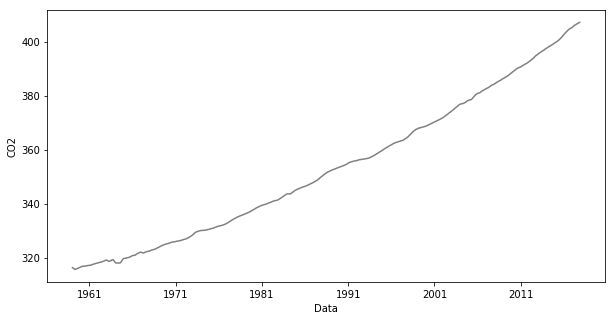
\includegraphics[width=.6\linewidth]{images/co2_filtered.png}
    \source{Elaborado pelo próprio autor a partir de \citeonline{co2data}}
\end{figure}

\subsubsection{Diferenciação}\label{sec:diff}

Outra tarefa a ser observada em relação ao entendimento de tendência é a forma na qual é removida. O método mais simples para remoção da tendência é subtrair de cada valor observado o valor do seu antecessor, conforme descrito na \autoref{eq:diferenciacao}. Normalmente, uma única diferenciação é suficiente para remover a tendência, porém em séries com componente sazonal podem vir a ser necessárias mais de uma em um \textit{lag} diferente.

\begin{equation}
    \label{eq:diferenciacao}
    y_t = x_t - x_{t-1}
\end{equation}


O gráfico da \autoref{fig:co2diff} mostra o resultado obtido para a série de leituras de $CO_2$ após uma diferenciação. 
%VALERIA: vc começou dizendo que a diferenciação serve para remover tendência e concluiu dizendo que a diferenciação evidenciou a componente sazonal (?!). Qual a relação? Além disso, por que esse gráfico evidencia a componente sazonal? Explique isso ao leitor.
Pelo gráfico é possível perceber que a série resultante se aproxima de uma série com função média constante, dando evidência a componente sazonal.

%Para dar um exemplo de diferenciação volto a série das leituras do $CO_2$ e agora realizando uma diferenciação, o resultado é visto na \autoref{fig:co2diff}, especificamente neste exemplo percebemos que a série se aproximou de uma série com função média constante, dando evidência a componente sazonal.

\begin{figure}
    \centering
    \caption{Série da leitura do $CO_2$ na atmosfera com uma
        diferenciação}\label{fig:co2diff}
    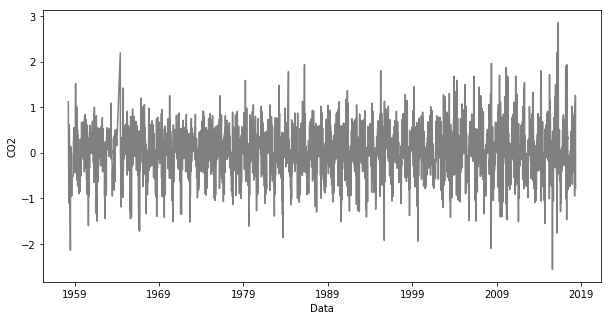
\includegraphics[width=.6\linewidth]{images/co2_diff.png}
    \source{Elaborado pelo autor a partir de \citeonline{co2data}}
\end{figure}

% \subsection{Sazonalidade}

% Conforme definido por \citeonline{ehlers} sazonalidade caracteriza repetições
% de comportamento de uma série em um período $s$ de tempo. Normalmente é
% facilmente observado na representação gráfica da série.

%VALERIA: PAREI REVISAR AQUI
\section{Modelos probabilísticos}

Como já disposto, as séries temporais podem ser previstas utilizando de modelos
estatísticos, isso segundo \citeonline{ehlers} ocorre devido ao seu caráter
estocástico por conta de cada observação possuir correlação com as observações
imediatamente antecessoras diferentemente de séries determinísticas, quais tem
seu estado definido por uma função matemática ou um sistema onde a saída só é
dependente das entradas atuais.

O modelo comumente utilizado para essa tarefa é o ARIMA, descrito por
\citeonline{box}, caracteriza a série em três parâmetros $(p,d,q)$, sendo cada
um associado a um processo, sendo $p$ associado a processos auto-regressivos,
$r$ a processos integrativos e $q$ a de médias móveis.

Para encontrarmos esses parâmetros \citeonline{box} descreveu alguns processos,
entre eles a analise da função de autocorrelação.

\subsection{Função de autocorrelação}\label{sec:corre}

Durante a parametrização precisaremos identificar o comportamento da série, uma
ferramenta para isso é a função de autocorrelação, com base na correlação entre
duas séries $X$ e $Y$, podemos obter a correlação de uma série com defasagem
$k$, sendo essa defasagem a distância entre o valor analisado $X_t$ a
observação $X_{t-k}$.

Assim podemos obter a função de autocorrelação para uma série de 100 elementos
ao considerar que a série $X$ é os 99 primeiros elementos e $Y$ os 99 últimos
elementos. Assim a função de autocorrelação será dada segundo
\autoref{eq:autocorrelacao}.

\begin{equation}
    \label{eq:autocorrelacao}
    r_k = \frac{\sum_{t=1}^{n-k}{(x_t - \overline{x})(x_{t+k} -
    \overline{x})}}{\sum_{t=1}^{n}{(x_t - \overline{x})^2}}
\end{equation}

Segundo \citeonline{ehlers} a função de autocorrelação quando plotada para os
$k$-ésimos primeiros coeficientes é chamado de correlograma e este é uma
ferramenta importante para as análises, como exemplo pode ser visto a
\autoref{fig:correlogramaCo2} na qual é disposto as 25 primeiras defasagens das
leituras de concentração de $CO_2$ na atmosfera, ainda segundo
\citeonline{ehlers} temos de definir ao correlograma o seu intervalo de
confiança, com o qual podemos considerar tudo que esteja acima desse como uma
correlação que deve ser analisada e abaixo desse limite será desconsiderada,
assim se todos as correlações estarem abaixo desse limite podemos considerar a
série como um ruído branco, para encontrar esse intervalo \citeonline{ehlers}
recomenda utilizar a seguinte equação $\pm{}1,96/\sqrt{n}$, sendo $n$ o número
de observações da série.

\begin{figure}
    \centering
    \caption{Gráfico da função de autocorrelação das leituras de
        $CO_2$}\label{fig:correlogramaCo2}
    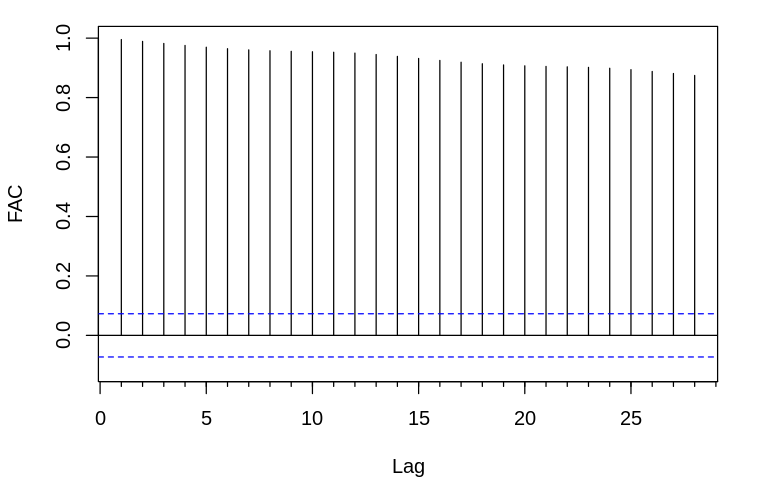
\includegraphics[width=.6\linewidth]{images/acf_co2.png}
    \source{Elaborado pelo autor a partir de \citeonline{co2data}}
\end{figure}

Pela \autoref{fig:correlogramaCo2} podemos concluir que as leituras do $CO_2$
apresentam uma tendência, e ainda por apresentar todos valores positivos
podemos afirmar que crescerá ao longo do tempo. Como a série possui tendência
temos de fazer uma diferenciação, como disposto na \autoref{sec:diff}, para
remoção dessa componente, vemos a série após essa diferenciação na
\autoref{fig:co2diff} e o correlograma após a diferenciação pode ser visto na
\autoref{fig:acfco2diff}, nesse novo gráfico é percebido que a componente da
tendência foi realmente removida após uma diferenciação, tornando visível a
componente sazonal, vemos isso pela alternância das correlações observadas no
correlograma.

\begin{figure}
    \centering
    \caption{Gráfico de função de autocorrelação da diferenciação da série de
        $CO_2$}\label{fig:acfco2diff}
    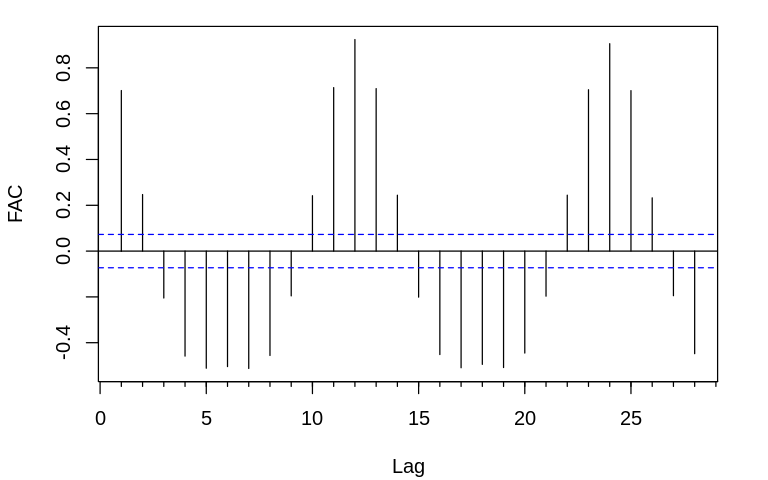
\includegraphics[width=.6\linewidth]{images/acf_co2_diff.png}
    \source{Elaborado pelo autor a partir de \citeonline{co2data}}
\end{figure}

% TODO: Citar as seções nas quais o correlograma é apresentada em outros
%cenários

\subsection{ARIMA}

O modelo ARIMA já introduzido na seção anterior possui três parâmetros
essenciais $(p,q,d)$ sendo $p$ repensável por definir o numero de observações
considerados no processo auto regressivo, $q$ o numero de diferenciações
necessárias para a remoção da tendencia e $d$ o numero de termos no processo de
medias móveis.

\subsubsection{AR -- Processo auto regressivo}

% TODO Melhor descrição da forma que é encontrado os coeficientes e a
% utilização do ACF e PACF para identificação do p

Segundo \citeonline{ehlers} um processo $X_t$ é chamado auto regressivo de
ordem $p$, ou $AR(p)$, quando temos $X_t$ dado segundo a
\autoref{eq:aregressivo}.

\begin{equation}
    \label{eq:aregressivo}
    X_t = \alpha_1X_{t-1}+\epsilon_t
\end{equation}

Como observado na \autoref{eq:aregressivo} é um modelo útil se for razoável
assumir que o valor atual depende somente de seus antecessores imediatos mais
um erro aleatório.

\subsubsection{MA -- Processo de médias móveis}

% TODO Melhor descrição da forma que é encontrado os coeficientes e a
% utilização do ACF e PACF para identificação do q

Segundo \citeonline{timeseriesExample} o processo de médias móveis é dado como
a média dos termos passados e correntes e pode ser descrito matematicamente
segunda a \autoref{eq:pmediasmoveis}.

\begin{equation}
    \label{eq:pmediasmoveis}
    X_t = \epsilon_t - \theta_1\epsilon_{t-1} - \theta_2\epsilon_{t-2} - \theta_{q}\epsilon_{t-q}
\end{equation}

Onde os valores de $\theta$ serão dados após análise da série.

\subsubsection{ARMA -- Modelo misto}

Combinando o processo AR e MA podemos obter um modelo extremamente útil para
descrever séries temporais. E a união dos modelos pode ser expressa pela
\autoref{eq:arma}.

\begin{equation}
    \label{eq:arma}
    X_t = \mu + \sum_{j=-q}^{q}\sum_{i = 1}^{p} \phi{}x_{t-i}+\epsilon_t+\sum{i = 0}{q}\theta_i\epsilon_{t-i}
\end{equation}

\subsubsection{Integração}

Em séries não estacionarias, segundo a definição dada na
\autoref{sec:estacionaria}, é necessário a transformação em uma série
estacionaria, isso pode ser simplesmente realizado utilizando o método descrito
na \autoref{sec:diferenciacao}, assim podemos aplicar de forma adequada o
procedimento de \citeonline{box} para produzir um modelo probabilístico que
poderá ser utilizado na atividade de previsão da série.

% TODO Referencias??
Normalmente uma diferenciação é suficiente para remover a tendencia de uma
série e a transformar em uma série estacionária, entretanto em séries que
apresentem a componente sazonal pode vir a ser necessária a aplicação de duas
ou mais diferenciações e em casos da aplicação de modelos SARIMA essa
diferenciação é aplicada com uma intervalo $l$, com esse valor sendo dado pela
sazonalidade da série.

\subsection{Seleção do modelo}

De acordo com \citeonline{box} a identificação do modelo pode ser feita
a partir da análise gráfica da FAC e PACF, podendo contar com a ajuda de outros
testes para validação da estacionariedade da série.

O modo que \citeonline{box} desenvolveu análise o comportamento da correlação
de forma que para identificar a ordem do AR, $p$, é suficiente analisar se o
gráfico do FAC apresenta decaimento exponencial e PACF apresenta uma quebra a
partir do elemento $p$ do gráfico. Já a identificação da ordem do processo de
médias móveis é feita de modo análogo, porem o $q$ é dado pela elemento que
apresenta a quebra no gráfico do FACP enquanto o gráfico do FAC apresenta
decaimento exponencial.

Se não for possível identificar a série a partir deste procedimento, pode ser
que a série apresente tendencia ou sazonalidade. No caso de existir tendência é
necessária a realização de uma ou mais diferenciação na série, $d$, com essa nova
série agora estacionaria é refeito as verificações e determinadas as ordens.

No caso acima o modelo obtido ou é da forma $AR(p)$ ou $MA(q)$ porem em casos
de modelos hibridos os gráficos devem apresentar comportamento de decaimento a
partir do $p$ para o FAC e $q$ para FACP\@.

Porem, segundo \citeonline{vinay} essa forma nos fornece modelos que servem
somente como uma boa aproximação, para determinação de um modelo realmente
eficiente pode ser necessário a execução de um grande número de testes
exaustivos e selecionar aquele modelo que apresente modelo parcimonioso e que
gere um bom resultado.

\subsection{Determinação dos coeficientes}
Por fim, para completa construção do modelo apresentado na \autoref{eq:arima} é
necessario a obtenção dos coeficientes tanto do processo autoregressivo tanto
do de médias movéis. Para essa tarefa \citeonline{vinay} apresenta a
\autoref{eq:coef} que serve tanto para determinação dos coeficientes de ambos
processos.

\begin{equation}
    \label{eq:coef}
    \alpha = inv(M_A^T M_A) M_A^T M_B
\end{equation}

A matriz $M_A$ e $M_B$ são dadas da seguinte forma.

\section{Aprendizado de Máquina}

Segundo \citeonline{machineLearning} aprendizado de máquina é descrito como a
habilidade de algorítimos reconhecer padrões em um conjunto de dados.

Essa detecção de padrões permitem, por exemplo, a realização das seguintes
atividades.
\begin{itemize}
    \item Classificação\\
        É a tarefa de mapear uma entrada a uma categoria, como no exemplo na classificação dos números, apresentada no início da seção. Podemos
        encontrar ainda exemplos do uso de aprendizado de máquina para
        classificação em diversos outros trabalhos, como
        \citeonline{artigoClassificacao} que utilizou redes neurais artificiais
        para realizar a classificação de imagens.
    \item Regressão\\
        Já a tarefa de regressão é aplicada quando precisamos mapear um
        conjunto de valores a uma saída em $ \mathbb{R} $,
        \citeonline{regressao} utilizou redes neurais artificiais para
        encontrar um modelo que permitisse a previsão da demanda de uso de
        energia elétrica, mapeando o carga atual e informações climáticas a
        carga futura.
\end{itemize}

E sendo ainda hoje considerada a era da informação, e os dados que antes eram
acessíveis somente a corporações estão hoje disponíveis, isso tudo acompanhado
do aumento de fonte dados que vão desde estatísticas de acessos a um site a
sensores espalhados pelo globo. Logo, o estudo desses dados e a capacidade de
se tomar decisões embasadas vem se tornando cada vez mais
relevante.\cite{ethem}

Um exemplo de uso de aprendizado de máquina é a identificação de caracteres
numéricos escritos a mão, esse exemplo é apresentado por
\citeonline{machineLearning} e o descreve como um problema de classificação no
qual uma imagem de dimensões $28 \times 28$ pixeis é dada como entrada em um
sistema e este deve atribuir uma classificação que descreve qual o número
que a figura representa, um conjunto de exemplo dessas imagens pode ser visto
na \autoref{fig:numeroClassi}.

\begin{figure}
    \centering
    \caption{Exemplo de entrada para o algorítimo de
        classificação}\label{fig:numeroClassi}
    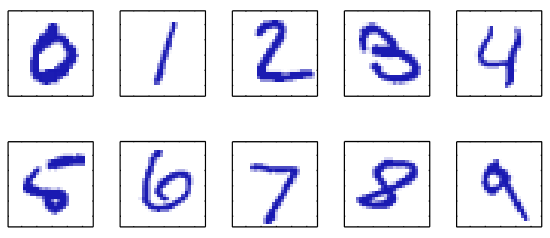
\includegraphics[width=.5\linewidth]{images/numeroClassificacao.png}
    \source{\citeonline{machineLearning}}
\end{figure}

No exemplo apresentado na \autoref{fig:numeroClassi} podemos entender a
atividade como um sistema onde $x$ é a entrada e $\hat{y}$ a saída do sistemas,
de forma matemática podemos expressar da forma vista na \autoref{eq:sisCla}. A
saída será na forma de um conjunto de números variando de 0 a 1 expressando a
probabilidade de $x$ pertencer a a classe $\hat{y}_i$ onde $i$ é o índice do
conjunto.

\begin{equation}
    \label{eq:sisCla}
    f(x) = \hat{y}
\end{equation}

\subsection{Redes Neurais artificiais}

Segundo \citeonline{haykin} a pesquisa em redes neurais artificiais é motivada
pelo entendimento que o cérebro humano realiza o processamento de uma forma
completamente diferente dos computadores convencionais. Essa forma de realizar
o processamento realizado pelo cérebro é altamente complexa, não linear e
altamente paralela. A unidade de processamento e organização básica de um
cérebro são os neurônios, o autor ainda lhe confere superior capacidade na
realização de tarefas como reconhecimento de padrões do que os computadores
digitais.

Os animais já nascem com o cérebro possuindo certa estruturas que estes vão
precisar durante sua vida, porem este é concebido ainda de maneira muito
plastica, ou seja, possuindo ainda a capacidade de na fase de aprendizado ser
capaz de se adaptar ao contexto em que vai se desenvolver. Este mesmo conceito
de plasticidade também será utilizado para a modelagem de redes neurais
artificiais~\cite{haykin}.

\subsubsection{\textit{Perceptron}}

Como já colocado, as redes neurais possuem o neurônio como elemento de
processamento, este em redes artificiais associamos ao \textit{perceptron},
descrito primeiramente por Rosenblatt em 1958, e tem sua função definida em
\autoref{eq:perceptron} sendo dado como a soma ponderada por $w_i$ das
entradas, $x_i$.

\begin{equation}
    \label{eq:perceptron}
    v = \sum_{i=1}^{m}{w_i + b}
\end{equation}

% TODO: Algorítimo
% TODO: MLP
% TODO: Back Propaggation
% TODO: Descida de Gradiente
% TODO: - Adam

\subsubsection{MLP}

\subsubsection{Adam}

\section{Métricas de avaliação}

\chapter{Desenvolvimento}\label{chap:desenv}

Para demonstrar e avaliar a capacidade de os métodos de previsão apresentados
neste trabalho, foi selecionada uma série temporal qual consta as vendas
diárias de uma rede de farmácias germânica, os dados foram obtidos
\textit{online}\footnote{Kaggle
    \url{https://www.kaggle.com/c/rossmann-store-sales}}.

Foram realizadas algumas etapas de pré processamento dos dados antes de
obtermos a série temporal efetivamente utilizada para a previsão.
Primeiramente foi necessária a seleção de uma loja aleatoriamente, já que o
conjunto de dados obtidos nos traz dados das diversas lojas que compõe a rede.
Foi selecionada então de forma aleatória a loja de ID 67. Após foi então obtida
uma série temporal multivariada, entretanto, a proposta deste trabalho é a
avaliação de previsões em séries uni variadas, ou seja, embora o conjunto de
entrada possua mais informação que aquelas que serão utilizadas para previsão,
estas serão descartadas. Logo a série será composta somente da quantidade
diária de vendas realizadas. O gráfico que apresenta a série a ser encontrado o
modelo é vista na \autoref{fig:serieRossman}.

\begin{figure}[ht]
    \centering
    \caption{Gráfico de observações das vendas diárias}\label{fig:serieRossman}
    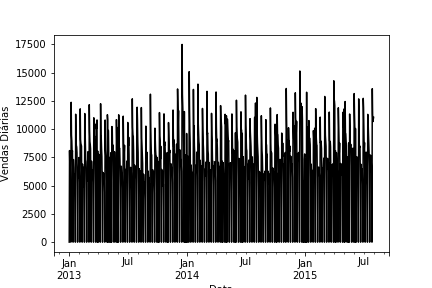
\includegraphics[width=.6\textwidth]{images/graficoRossman.png}
    \source{Elaborado pelo autor}
\end{figure}

\begin{figure}[ht]
    \centering
    \caption{Gráfico contendo 3 semanas de observações para visualização do
        comportamento semanal da série}\label{fig:serieRossmanSemana}
    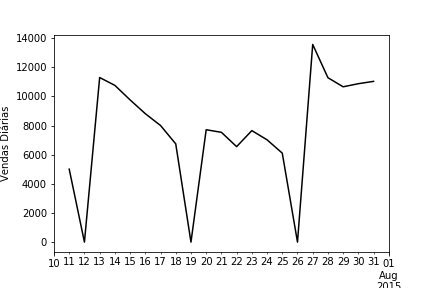
\includegraphics[width=.6\textwidth]{images/graficoRossmanSemana.png}
    \source{Elaborado pelo autor}
\end{figure}

Observamos na \autoref{fig:serieRossman} a existência de valores que podem ser
descritas como \textit{outliers}, isto é, são leituras que estão fora do padrão
esperado, isso ocorre devido às observações serem diárias e a rede de farmácia
não possuir expediente aos domingos, pode ser visto de forma mais clara na
\autoref{fig:serieRossmanSemana}, nesses dias as leituras aparecerão zeradas e
assim gerando uma série que embora com maior número de observações possuirá
instabilidade, que aumenta consideravelmente a complexidade do modelo, para
evitar esse problema foi realizada a conversão para observações semanais,
somando a quantidade de vendas realizada em uma semana em um único valor, essa
nova série é apresentada na \autoref{fig:serieRossmanSemanal}.

\begin{figure}[ht]
    \centering
    \caption{Gráfico de observações semanais de
        vendas}\label{fig:serieRossmanSemanal}
    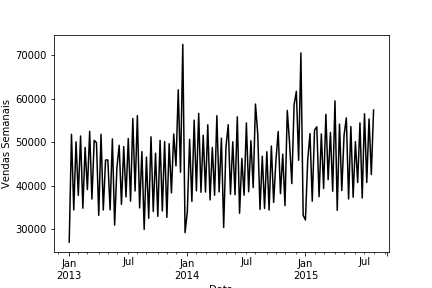
\includegraphics[width=.6\textwidth]{images/graficoRossmanSemanal.png}
    \source{Elaborado pelo autor}
\end{figure}

\section{Análise da série}

Para continuarmos com a parametrização dos modelos que serão avaliados temos de
ter uma boa compreensão do comportamento da série, para isso são aplicadas
algumas ferramentas apresentados como o correlograma descrito na
\autoref{sec:corre}.

Em primeira analise observamos na \autoref{fig:serieRossmanSemanal} que em dois
momentos a série apresenta máximos locais, observado de forma detalhada na
\autoref{fig:rossmanFimAno}.

\begin{figure}
    \centering
    \caption{Gráfico do comportamento da série no fim do
        ano}\label{fig:rossmanFimAno}
    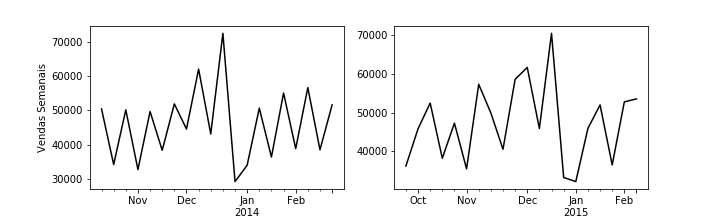
\includegraphics[width=.8\textwidth]{images/graficoRossmanFimAno.png}
    \source{Elaborado pelo autor}
\end{figure}

O conjunto de dados utilizado, ainda nos trás outras informações, como se houve
promoção naquele dia ou se foi feriado. Se considerarmos essas informações
podemos compreender algumas flutuações que ocorrem na série, por exemplo se
observarmos a \autoref{fig:rossmanPromo} vemos que os maiores volumes de venda
tendem a ocorrer nos dias de promoção.

% TODO: Gerar essa imagem
\begin{figure}
    \centering
    \caption{Observações marcados conforme ocorrência de promoções}
    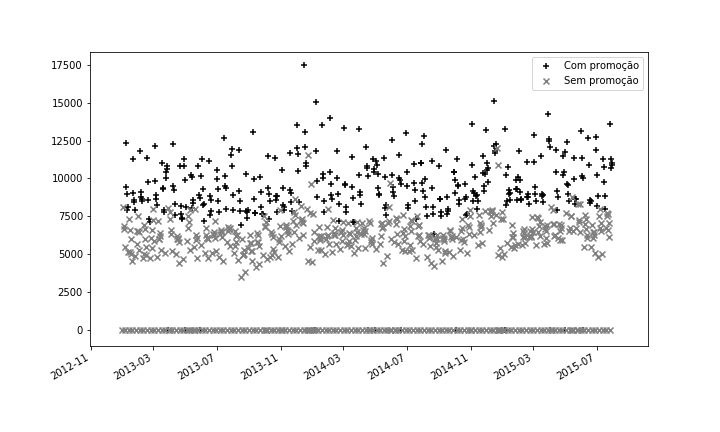
\includegraphics[width=.7\textwidth]{images/graficoRossmanPromo.png}
    \source{Elaborado pelo autor}
\end{figure}

Aplicando então a função de autocorrelação apresentada anteriormente obteremos
informações para a parametrização do modelo, utilizando a série com frequência
semanal apresentado na \autoref{fig:serieRossmanSemanal} teremos a seguinte
\autoref{fig:acfRossmanSemanl}.

% \begin{figure}
%     \centering
%     \caption{Função de Autocorrelação aplicada a série}
%     \includegraphics[width=.7\textwidth]{images/graficoAcfSemanal.png}
%     \source{Elaborado pelo autor}
% \end{figure}

\section{Aprendizado de máquina}

Diferentementr do ARIMA, redes neurais artificiais não foram elaboradas com a
r: target STRING not available

visão na aplicação de previsão de séries temporais, na verdade seu uso é muito
mais abrangente que este, no entanto, se considerarmos o problema de previsão
de redes neurais como um problema de regressão poderemos modelar a rede neural
para que a saída desta seja a próxima observação da série.

A entrada da rede neural foi estabelecida como duas observações no passado,
porem poderia ser utilizado mais, mas para manter o modelo parcimonioso foi
mantido assim.

Na etapa de escolha dos parâmetros foi utilizado busca em grade com validação
cruzada, com \textit{fold} de tamanho cinco. Os parâmetros testados estão
apresentas na \autoref{tab:grid}, para validação do modelo foi calculado o MAPE
e então selecionado aquele que melhor representou a série.

\begin{table}
    \centering
    \caption{Parâmetros testados na busca em grade}\label{tab:grid}
    \begin{tabular}{ l r }
        \toprule
        Parâmetros                      & Valores testados\\
        \midrule
        Número de camadas escondidas    & [1, 2, 3, 4]\\
        Número de neurônios por camadas & [2, 4, \ldots, 100]\\
        Função de ativação              & [relu, tanh]\\
        Número de épocas                & [500, 1000, 1500]\\
        Otimizador                      & [adam, sgd]\\
        \bottomrule
    \end{tabular}
    \source{Elaborado pelo autor}
\end{table}

Após execução, o resultado da busca em grade retornou que a melhor escolha a
utilização de somente uma camada escondida com 12 neurônios, alem disso a
função de ativação ficou estabelecida como a relu, com otimização usando adam.
A arquitetura da rede neural resultante é demonstrada na
\autoref{fig:redeNeural}.

\begin{figure}
    \centering
    \caption{Representação gráfica da rede neural artificial utilizada para
        avaliação}\label{fig:redeNeural}
    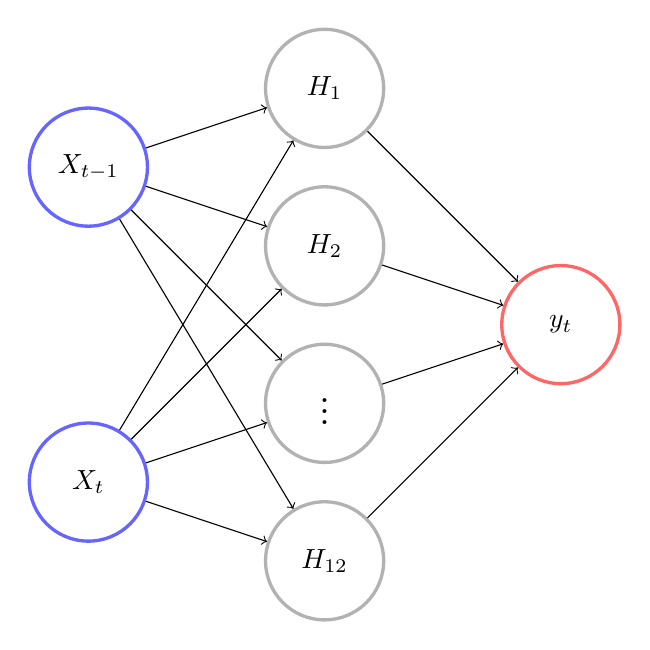
\begin{tikzpicture}[
            neuron/.style={circle, very thick, minimum size=15mm},
            input/.style={draw=blue!60},
            hidden/.style={draw=gray!60},
            output/.style={draw=red!60},]

        % Nodes entrada
        \node[neuron, input]  (entrada1)   at (0, 5cm)   {$X_{t-1}$};
        \node[neuron, input]  (entrada2)   at (0, 1cm)   {$X_{t}$};

        % Nodes escondidos
        \node[neuron, hidden] (escondido1) at (3cm, 6cm) {$H_1$};
        \node[neuron, hidden] (escondido2) at (3cm, 4cm) {$H_2$};
        \node[neuron, hidden] (escondido3) at (3cm, 2cm) {$\LARGE{\vdots}$};
        \node[neuron, hidden] (escondido4) at (3cm, 0)   {$H_{12}$};

        % Nodes Saída
        \node[neuron, output] (saida)      at (6cm, 3cm) {$y_t$};

        \foreach \dest in {1,...,4}
            \path[->] (entrada1) edge (escondido\dest);

        \foreach \dest in {1,...,4}
            \path[->] (entrada2) edge (escondido\dest);

        \foreach \dest in {1,...,4}
            \path[->] (escondido\dest) edge (saida);
    \end{tikzpicture}
    \source{Elaborado pelo autor}
\end{figure}

\chapter{Resultados}\label{chap:result}

\chapter{Conclusões}\label{chap:concl}

\section{Trabalhos futuros}

\postextual

\bibliography{referencias}

\end{document}
